\documentclass[letterpaper,11pt]{article}

% Soporte para los acentos.
\usepackage[utf8]{inputenc}
\usepackage[T1]{fontenc}
% Idioma español.
\usepackage[spanish,mexico, es-tabla]{babel}
% Soporte de símbolos adicionales (matemáticas)
\usepackage{multirow}
\usepackage{amsmath}
\usepackage{amssymb}
\usepackage{amsthm}
\usepackage{amsfonts}
\usepackage{mathtools}
\usepackage{latexsym}
\usepackage{enumerate}
\usepackage{ragged2e}
\usepackage{listings}
\usepackage{xcolor}
\usepackage{graphicx}
\usepackage{hyperref}
% Modificamos los márgenes del documento.                                       %
\usepackage[lmargin=2cm,rmargin=2cm,top=2cm,bottom=2cm]{geometry}

\definecolor{codegreen}{rgb}{0,0.6,0}
\definecolor{codegray}{rgb}{0.5,0.5,0.5}
\definecolor{codepurple}{rgb}{0.58,0,0.82}
\definecolor{backcolour}{rgb}{0.95,0.95,0.92}

\lstdefinestyle{mystyle}{
    backgroundcolor=\color{backcolour},   
    commentstyle=\color{codegreen},
    keywordstyle=\color{magenta},
    numberstyle=\tiny\color{codegray},
    stringstyle=\color{codepurple},
    basicstyle=\ttfamily\footnotesize,
    breakatwhitespace=false,         
    breaklines=true,                 
    captionpos=b,                    
    keepspaces=true,                 
    numbers=left,                    
    numbersep=5pt,                  
    showspaces=false,                
    showstringspaces=false,
    showtabs=false,                  
    tabsize=2
}

\lstset{style=mystyle}

\title{Facultad de Ciencias, UNAM \\ Redes Neuronales \\ Tarea 5}
\author{Rubí Rojas Tania Michelle}
\date{1 de junio de 2020}

\begin{document}
\maketitle

\begin{enumerate}
    % Ejercicio 1.
    \item Construye una red neuronal convolucional para detectar las imágenes
    en el \textit{dataset} de perros y gatos. 

    \textsc{Solución:} Primero, descomprimimos cada uno de nuestros archivos 
    \textit{.zip} y los almacenamos en una carpeta llamada \textit{dataset}:
    \begin{lstlisting}[language=Python]
    import os
    from zipfile import ZipFile

    # Le hacemos un unzip a nuestro conjunto de entrenamiento.
    with ZipFile('dataset/train_dogscats.zip', 'r') as zipObj:
        zipObj.extractall('dataset')

    # Le hacemos un unzip a nuestro conjunto de prueba.
    with ZipFile('dataset/test_dogscats.zip', 'r') as zipObj:
        zipObj.extractall('dataset')
    \end{lstlisting}

    Creamos un \textit{dataframe} con cada una de las imágenes dentro de la 
    carpeta \textit{train}. Como el nombre de cada imagen nos indica si el 
    animalito es un perro o es un gato, extraeremos esa información.
    \begin{lstlisting}[language=Python]
    import pandas as pd 

    # Obtenemos el nombre de cada uno de los archivos que estan en train.
    nombres = os.listdir("dataset/train")

    categoria = []
    for nombre in nombres:
        animal = nombre.split('.')[0]  # Obtenemos el nombre del animalito.
        if animal == 'dog':
            categoria.append(1)
        else:
            categoria.append(0)

    datafr = pd.DataFrame({'nombres': nombres, 
                        'categoria': categoria
                        })

    # Visualizamos el dataframe con 10 archivos.
    datafr.head(10)
    \end{lstlisting}

    \begin{figure}[ht]
        \centering
        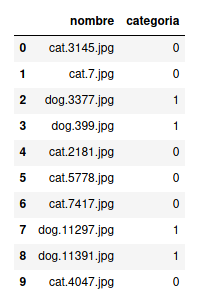
\includegraphics[width=0.3\textwidth]{./imagenes/dataframe.png}
    \end{figure} 

    \newpage
    Así, tenemos un \textit{dataframe} con cada una de las imágenes y sus 
    respectivas etiquetas.

    % Ejercicio 2.
    \item ¿Qué arquitectura diseñaste?
    
    \textsc{Solución:}

    % Ejercicio 3.
    \item Haz las gráficas de pérdida y de precisión tanto para el entrenamiento
    como para la validación y preséntalas.

    \textsc{Solución:}

    % Ejercicio 5.
    \item Úsalo para reconocer las $4$ imágenes anexas.
    
    \textsc{Solución:}
\end{enumerate}

\end{document}